\definecolor{green}{RGB}{0,128,0}
  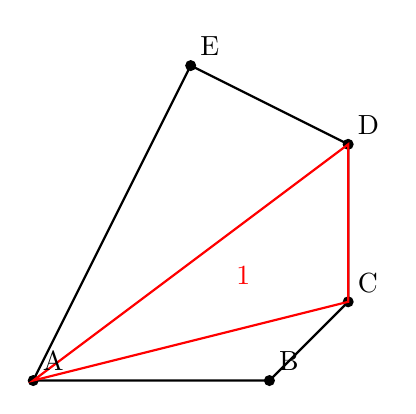
\begin{tikzpicture}
    % Define the points
    \coordinate (A) at (0,0);
    \coordinate (B) at (3,0);
    \coordinate (C) at (4, 1);
    \coordinate (D) at (4,3);
    \coordinate (E) at (2,4);
    
    % Draw the points
    \foreach \point in {A,B,C,D,E}
      \fill (\point) circle (2pt);

    \draw[thick] (A) -- (B) -- (C) -- (D) -- (E) -- cycle;
    \draw[thick,red] (A) -- (C) -- (D) -- cycle;

    \coordinate (CenterACD) at (barycentric cs:A=1,C=1,D=1);
    \node[red] at (CenterACD) {1};


    
    % Label the points
    \node[above right] at (A) {A};
    \node[above right] at (B) {B};
    \node[above right] at (C) {C};
    \node[above right] at (D) {D};
    \node[above right] at (E) {E};

    \end{tikzpicture}
